\documentclass[]{standalone}
\usepackage{tikz}
\usetikzlibrary{shapes,arrows,calc,positioning}
\usepackage{amsmath} % for dfrac
\usepackage{comment}
\usepackage{calc}

\tikzstyle{note} = [draw, ellipse, node distance=3.5cm, minimum height=1em, text width=8cm, text centered]

\begin{document}
	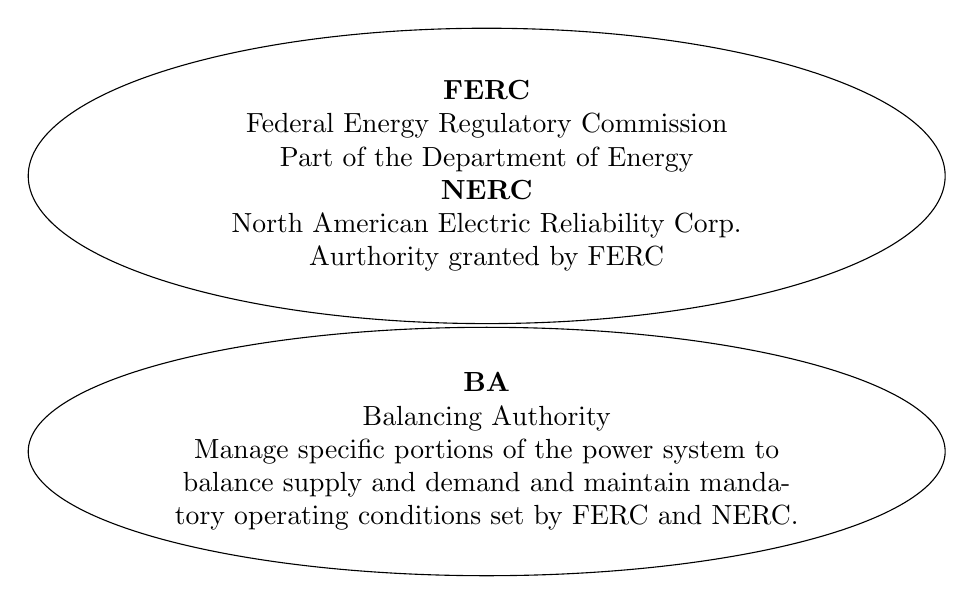
\begin{tikzpicture}[auto,>=triangle 45]
		\node[note] (theman) {{\textbf{FERC} \\ Federal Energy Regulatory Commission \\
		Part of the Department of Energy}
		{\\\textbf{NERC} \\ North American Electric Reliability Corp.\\
		Aurthority granted by FERC}}; 
		
		
		
		\node[note,below of=theman] (ba) {{\textbf{BA} \\ Balancing Authority \\
		Manage specific portions of the power
		system to balance supply and demand
		and maintain mandatory operating
		conditions set by FERC and NERC.}}; 
		
	\end{tikzpicture} 
\end{document}